\documentclass[conference]{IEEEtran}
\IEEEoverridecommandlockouts

\usepackage{cite}
\usepackage{amsmath,amssymb}
\usepackage{graphicx}
\usepackage{booktabs}
\usepackage{url}
\usepackage[hidelinks]{hyperref}

% Minimal pseudocode float. The algorithm/algorithmic packages are not in every
% TeX installation this is built on, and an eight-line skeleton does not justify
% the dependency.
\newcounter{algo}
\newcommand{\aln}[2]{\makebox[1.5em][r]{\scriptsize#1:}\hspace{.45em}#2\par}
\newcommand{\alnx}[1]{\makebox[1.5em][r]{}\hspace{.45em}#1\par}
\newcommand{\ind}{\hspace*{1.2em}}
\newcommand{\cmt}[1]{{\footnotesize\itshape\quad$\triangleright$~#1}}
\newenvironment{algo}[1]{%
  \begin{figure}[t]\refstepcounter{algo}\small
  \setlength{\parindent}{0pt}\setlength{\parskip}{1.6pt}%
  \hrule height .9pt \vspace{3pt}
  \textbf{Algorithm \thealgo}\quad #1\par
  \vspace{2.5pt}\hrule height .4pt \vspace{4pt}}%
  {\vspace{3.5pt}\hrule height .9pt \end{figure}}

\begin{document}

\title{Sampling-Based Predictive Control for Obstacle Avoidance\\
with an Underactuated Triple-Pendulum Cartpole}

\author{\IEEEauthorblockN{William Xie}
\IEEEauthorblockA{Department of Computer Science\\
University of Colorado Boulder\\
Boulder, CO, USA\\
william.xie@colorado.edu}}

\maketitle

\begin{abstract}
We measure how far simple sampling-based model-predictive control gets on an
obstacle-avoidance task with chaotic, underactuated dynamics: a three-link
pendulum on a cart, one actuator for four degrees of freedom, that must drive
through gaps narrower than the pendulum is long. Six MJPC planners are compared
at equal iteration budget on a single bottleneck and on three chained
bottlenecks, under a collision test that allows no penetration at all. On one
bottleneck the best planner reaches 76/100; on three, the best reaches 4/100 and
five of the six never succeed. A memoryless control that discards its incumbent
each iteration solves none of 300 trials, placing the warm start rather than the
update rule at the centre of what these planners do. We then sweep the two
parameters of the avoidance
cost --- its weight and the clearance margin at which it activates --- over
$5\times5$ configurations, three seeds each, 50 trials per cell. The two do not
act independently: the surface is a ridge, and following it raises the same
planner from 2.7\% to 54\% on the three-bottleneck course. Extending the sweep
by a further $64\times$ in weight and down to a $0.01$~m margin follows the
ridge to 65\% (95\% CI 57--72), with the best margin sliding down as the weight
rises and the gain per factor of four falling below what 150 trials per cell
can resolve. Widening the search from 10 rollouts per iteration to 40 --- one
integer in the task file, and the budget annealed sampling already spends ---
adds a further 20 points to 85\% (79--90), at $2.65\times$ the wall time rather
than $4\times$, because 10 rollouts could not fill the thread pool. Eighty adds
nothing. At that matched budget the plain sampler beats annealed sampling by 22
points, and annealed sampling on 40 rollouts is indistinguishable from the plain
sampler on 10, so the annealing schedule converts a fourfold budget into nothing
measurable. Carrying the plan forward by shifting and extending it instead of
resampling it is a wash. We report per-iteration cost,
control effort and cost share for every configuration, and single-thread and
multi-thread planning throughput on two hosts at both rollout counts. We also report a negative result
for AgileRRT, the sample-based planner this task was originally built for, and
for iLQG, whose finite-difference derivatives dominate its cost while its
linearization is invalidated by contact. All figures in this report were
produced by seeded runs whose exact command lines are recorded alongside them.
\end{abstract}

\begin{IEEEkeywords}
model predictive control, sampling-based optimization, obstacle avoidance,
underactuated systems, MuJoCo
\end{IEEEkeywords}

\section{Introduction}

Predictive control with a physics engine in the loop is now cheap enough to run
online, and MJPC \cite{mjpc} makes the comparison between planners concrete: one
task specification, one rollout budget, several optimizers behind the same
interface. What it does not settle is which problems the derivative-free
planners can actually close, and what determines the boundary.

This report characterizes that boundary on one task. The system is the
three-link pendulum cartpole of Caldwell and Correll \cite{caldwell2015}, which
has four degrees of freedom, one actuator, chaotic passive dynamics, and an
obstacle gap half the pendulum's length. Passing the gap requires laying the
pendulum out near-horizontal, driving through, and recovering --- a maneuver that
cannot be held open-loop and that a single contact disqualifies.

We report three things.

First, a planner comparison at fixed iteration budget on one bottleneck and on
three, under a zero-tolerance collision test. The ordering is stable across both
worlds, but the success rates are not: three chained gaps take the best planner
from 76/100 to 4/100.

Second, a two-parameter sweep of the avoidance cost. The weight and the
clearance margin are the only knobs in the cost that concern the obstacles, and
they are not interchangeable: weight sets what a violation costs, margin sets
how early the cost arrives. Mapped over $5\times5$ values with three seeds per
cell, the success rate on the three-bottleneck course is not a monotone function
of either: the surface is a ridge, and the best margin slides down as the weight
rises. Following it past the first grid reaches 65\%, an order of magnitude above
the default.

Third, the width of the search itself. Holding the objective at the best ridge
cell and raising the rollouts per planning iteration from 10 to 40 reaches
85\%. This is a single integer in the task file rather than an algorithm, it is
the second largest effect we measured, and it is the same rollout budget that
annealed sampling has been spending on its annealing schedule throughout.
Eighty rollouts adds nothing.

Fourth, the cost of running any of this: per-iteration wall time by planner,
where that time goes, control effort and per-term cost share for the surviving
configurations, and throughput on an Intel Core Ultra 7 265KF and an Apple M5
Pro.

We also record two negative results, because both were measured rather than
assumed: AgileRRT does not fit a receding-horizon budget by three orders of
magnitude, and iLQG is the weakest planner here for reasons that are structural.

\begin{figure*}[t]
\centering
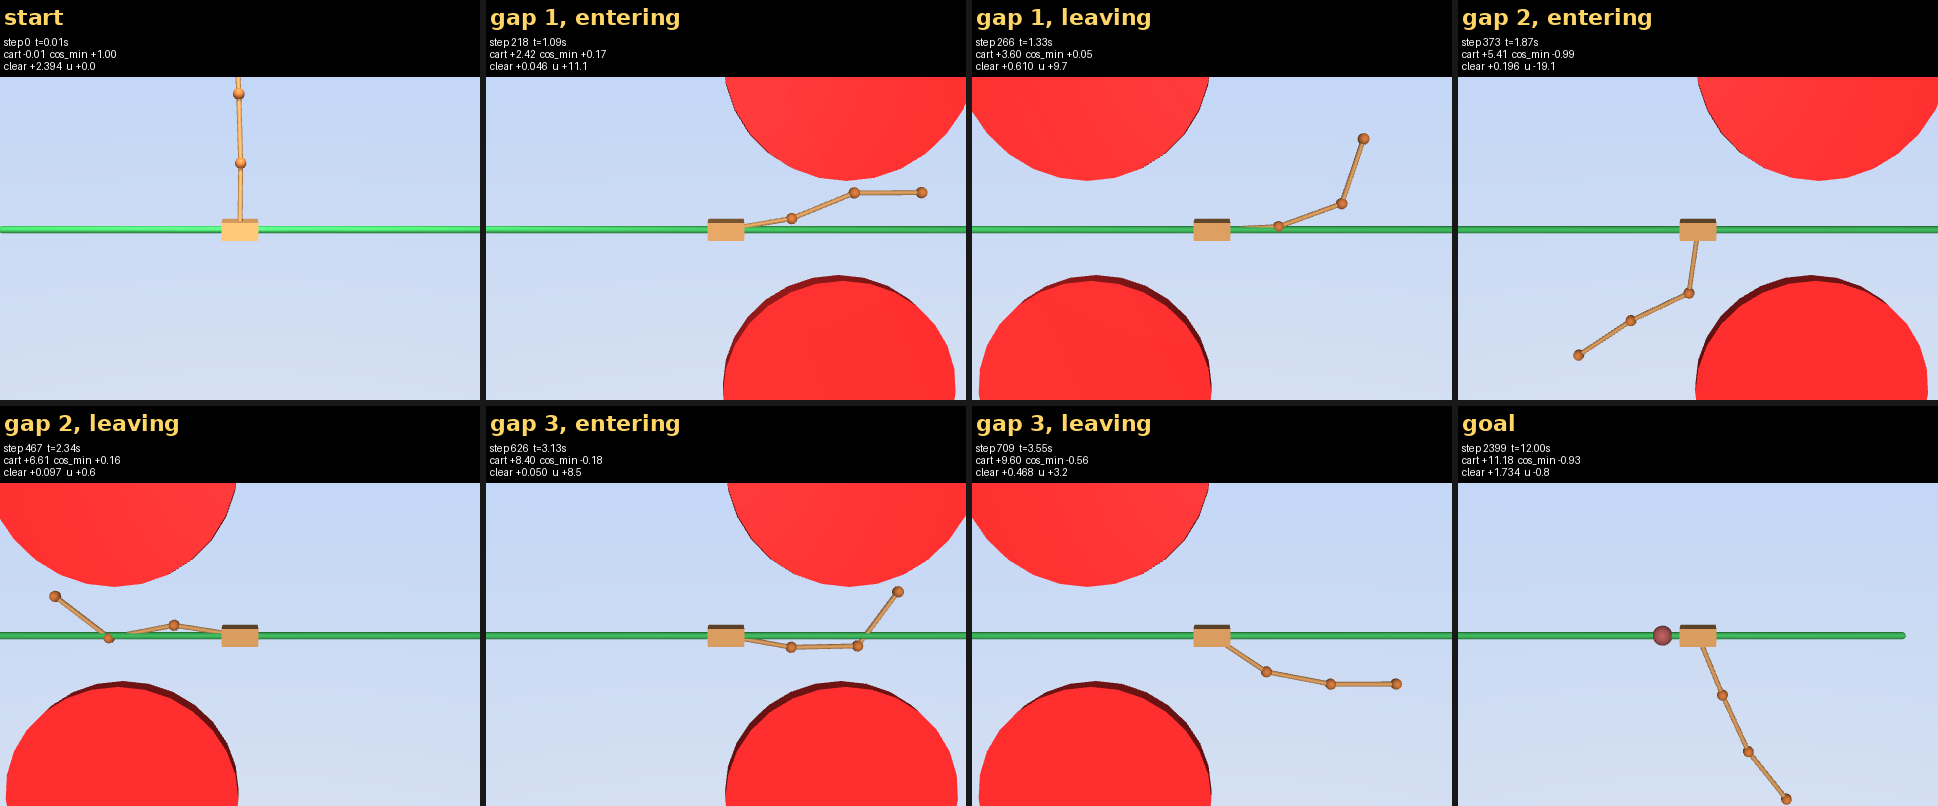
\includegraphics[width=\textwidth]{fig/filmstrip_solved.png}
\caption{One clean slalom solve, predictive sampling at avoidance weight
$128{,}000$ and margin $0.04$~m, seed $1000$. The camera tracks the cart, and
panels are placed at the events that decide the run rather than at uniform
intervals. Each panel reports the step, simulated time, cart position,
$\min_i \cos\theta_i$, the minimum head-to-disk clearance $\min_{ij} d_{ij}$ in
metres, and the applied force. Top row: the start, upright; the swing-down at
$t = 0.33$~s; the tightest moment of the run at $t = 1.12$~s, $27$~mm of
clearance inside the first gap; clear of it at $t = 1.20$~s. Bottom row: the
second and third crossings at $t = 2.14$ and $3.31$~s, both with $27$~cm of
clearance; the goal reached at $t = 4.82$~s; and the run parked at $t = 12$~s.
At all three crossings the links are laid out along the rail at hub height,
which is the posture that fits a $0.5$~m gap --- the cart passes the gap while
the pendulum is horizontal, and the run is decided by whether the swing phase
happens to place it there.}
\label{fig:filmstrip}
\end{figure*}

\section{Task}

\subsection{System}

A cart of mass $1.0$~kg slides on a horizontal rail. Attached to it is a
three-link pendulum; each link is a massless rod of length $L = 1/3$~m carrying
a point mass of $0.1$~kg at its tip, modelled as a sphere of radius
$\rho = 0.028$~m. The single actuator applies a horizontal force to the cart,
$|u| \leq 20$~N. There is no joint damping and no friction. With
$q = (x_{\text{cart}}, \theta_1, \theta_2, \theta_3)$ the system has $n_q = 4$,
$n_v = 4$, $n_u = 1$. Angles follow the reference implementation: $\theta_i = 0$
points link $i$ along $+z$, so head $i$ sits at
\begin{equation}
p_i = \Big(x_{\text{cart}} + L\!\!\sum_{j\le i}\!\sin\theta_j,\;\;
           L\!\!\sum_{j\le i}\!\cos\theta_j\Big).
\end{equation}
Physics is integrated by MuJoCo \cite{mujoco} with
\texttt{implicitfast} at $\Delta t = 5$~ms.

\subsection{Two worlds}

Obstacles are cylinders of radius $R = 0.6$~m with axis along $y$, so in the
$xz$ plane they are disks. They are real collision geoms, not merely cost
terms.

\emph{Corridor} is the task of \cite{caldwell2015}, \S5: one pair of disks at
$x = 3$, $z = \pm 0.85$, leaving a gap of
$2(0.85 - 0.6) = 0.5$~m, and a goal at $x = 6$. The pendulum is $1.0$~m long, so
it cannot pass upright.

\emph{Slalom} keeps that bottleneck unchanged and adds two more at $x = 6$ and
$x = 9$, with the goal at $x = 11$. The gaps are identical and the spacing is
$3$~m, which is $0.8$--$1.0$~s of travel at the speeds the cart reaches and
therefore straddles the $1$~s planning horizon. Because the first bottleneck is
the corridor task's exactly, the difference between results on the two worlds is
attributable to what follows it.

\subsection{Success criterion}

A trial is a \emph{solve} if the cart ends within $0.3$~m of the goal and no
head ever overlapped a disk. The pendulum's terminal configuration is not
scored, because the objective used throughout gives the upright term zero
weight: requiring an upright finish would score a run against a term it was
never given.

The collision test admits no penetration. An earlier version of this benchmark
allowed $20$~mm, on the theory that soft contacts permit a few harmless
millimetres on touch. Two measurements retract it. Across 30 recorded rollouts,
\texttt{ncon > 0} and $\min_i d_i < 0$ agree on every step --- MuJoCo never
reports contact between separated geoms, so there is no grazing band to protect.
And measured penetrations run continuously from $2$ to $39$~mm, so no depth
threshold separates numerical from real. At $20$~mm on a $28$~mm head, a sphere
71\% inside a disk scored as clean. We report both criteria in
Section~\ref{sec:planners-one} and \ref{sec:planners-three}, because the gap
between them is itself informative, but the zero-tolerance column is the result.

\section{Predictive control formulation}

\subsection{Objective}

We follow MJPC's formulation \cite{mjpc}. A task is specified by a residual
vector $r(x,u)$ partitioned into $M$ terms, each with a norm $n_i$ and a weight
$w_i$; the running cost is
\begin{equation}
c(x,u) \;=\; \sum_{i=1}^{M} w_i \, n_i\!\left(r_i(x,u)\right),
\label{eq:cost}
\end{equation}
and every term here uses the quadratic norm $n_i(r) = \tfrac{1}{2}\|r\|_2^2$.
At each control step the planner minimizes the mean running cost over a horizon
of $T$ steps,
\begin{equation}
J(u_{0:T-1}) \;=\; \frac{1}{T}\sum_{t=0}^{T-1} c(x_t, u_t),
\qquad x_{t+1} = f(x_t, u_t),
\label{eq:objective}
\end{equation}
with $x_0$ the current state and $f$ one call to \texttt{mj\_step}. The control
sequence is not free: it is the sampling of a linear spline with $K = 12$ knots
over the horizon, so the decision variable is $\theta \in \mathbb{R}^{K n_u}$
and $u_t = \mathrm{spline}(\theta; t)$. With $T_h = 1.0$~s this is $83$~ms of
knot spacing. The first control of the optimized sequence is applied, the spline
is shifted forward, and the next iteration warm-starts from it.

\subsection{Cost terms}

Table~\ref{tab:terms} lists the five residual terms. The weights are stated on
the command line for every result in this report, so each table says what was
optimized.

\begin{table}[t]
\caption{Residual terms. $N$ is the number of disks: 2 on the corridor, 6 on the
slalom.}
\label{tab:terms}
\centering
\begin{tabular}{@{}llp{4.1cm}@{}}
\toprule
Term & dim & residual \\
\midrule
Cart      & 1        & $x_{\text{cart}} - x_{\text{goal}}$ \\
Upright   & 3        & $\cos\theta_i - 1$ \\
Velocity  & 4        & $\dot q$ \\
Control   & 1        & $u$ \\
Avoidance & $3N$     & $\max(0,\; \delta - d_{ij})$ \\
\bottomrule
\end{tabular}
\end{table}

The upright residual is written $\cos\theta_i - 1$ rather than $\theta_i$
because it is zero exactly at the upright equilibrium and smooth across the
$\pm\pi$ wrap, so the planner never sees a discontinuity manufactured by angle
unwrapping.

\subsection{Avoidance residual}
\label{sec:avoidance}

Clearance between head $i$ and disk $j$ is surface-to-surface in the $xz$ plane,
\begin{equation}
d_{ij}(x) \;=\; \big\| p_i(x) - o_j \big\|_2 \;-\; R_j \;-\; \rho_i,
\label{eq:clearance}
\end{equation}
so $d_{ij} = 0$ means touching. The avoidance residual is a hinge on it,
\begin{equation}
r^{\text{avoid}}_{ij}(x) \;=\; \max\!\big(0,\; \delta - d_{ij}(x)\big),
\label{eq:hinge}
\end{equation}
with $\delta$ the \emph{clearance margin}. Combined with the quadratic norm and
weight $w_{\text{avoid}}$, the avoidance term contributes
$\tfrac{1}{2} w_{\text{avoid}} \sum_{ij} \max(0, \delta - d_{ij})^2$: exactly
zero when every head is more than $\delta$ from every disk surface, and growing
quadratically inside that band.

Two properties of \eqref{eq:hinge} matter for the rest of this report.

The term exists to give the sampler a gradient \emph{before} contact. Contact
alone is a discontinuity in the rollout cost, and a sampler that only learns
about a disk by hitting it learns too late to steer around it. The cost is what
converts the obstacle into something the sampler can see at a distance.

And $\delta$ and $w_{\text{avoid}}$ do different things. The weight sets how much
a violation costs; the margin sets how early the cost arrives, which is the only
one of the two that buys the planner time. The half-gap is $0.25$~m, so a margin
approaching that makes the hinge active across the entire gap: even a head
travelling exactly down the centreline is inside the penalty, and the barrier
around each disk becomes a wall across the corridor. Section~\ref{sec:landscape}
measures where that transition happens.

\subsection{Planners: one loop, three branch points}
\label{sec:planners}

All six planners share the interface, the rollout budget, and the objective.
Five of the six also share a loop, and it is worth writing that loop out
because the differences between them are smaller than their names suggest.

Start from the simplest. \emph{Random Sampling} has no state: every iteration it
draws $n$ control splines from a fixed Gaussian centred on zero control, rolls
each out, keeps the cheapest, applies its first control, and throws the rest
away. There is no warm start and nothing carries between iterations. It is a
control rather than a proposal --- the gap between it and any planner that does
keep state is the measured value of keeping state.

\emph{Predictive Sampling} \cite{mjpc} changes exactly one thing: it centres the
draw on the incumbent $\theta$ rather than on zero, and keeps the incumbent
itself as one of the $n$ candidates so the update can never move uphill. Every
remaining sampling planner here is a further change to one of three choices in
the same loop --- where the samples are centred, how they are spread, and how
the winner is folded back into the incumbent. Algorithm~\ref{alg:skeleton}
writes the loop with those three as named functions; Table~\ref{tab:planners}
gives each planner's instantiation.

\begin{algo}{One planning iteration, shared by five of the six planners.}
\label{alg:skeleton}
\alnx{\textbf{Input:} incumbent $\theta$, state $x_0$, budget $n$, horizon $T$}
\aln{1}{$\bar\theta \leftarrow \textsc{Centre}(\theta)$ \cmt{what to sample around}}
\aln{2}{\textbf{for} $k = 1 \dots n$ \textbf{do}}
\aln{3}{\ind $\epsilon^{(k)} \sim \mathcal{N}(0, \Sigma^{(k)})$ \cmt{\textsc{Spread}}}
\aln{4}{\ind $\theta^{(k)} \leftarrow \bar\theta + \epsilon^{(k)}$}
\aln{5}{\ind $u_t \leftarrow \mathrm{spline}(\theta^{(k)}; t)$, roll out $f$ from $x_0$}
\aln{6}{\ind $J^{(k)} \leftarrow \frac{1}{T}\sum_{t<T} c(x_t, u_t)$ \cmt{Eq.~\eqref{eq:objective}}}
\aln{7}{\textbf{end for}}
\aln{8}{$\theta \leftarrow \textsc{Fold}\big(\{\theta^{(k)}\}, \{J^{(k)}\}\big)$ \cmt{how the winner is kept}}
\aln{9}{apply $\mathrm{spline}(\theta;0)$; shift $\theta$ forward one step}
\end{algo}

\begin{table}[t]
\caption{How each planner instantiates Algorithm~\ref{alg:skeleton}. $\sigma$ is
the sampling standard deviation in newtons against a $\pm 20$~N actuator.
Rollouts are per planning iteration.}
\label{tab:planners}
\centering
\small
\begin{tabular}{@{}llll r@{}}
\toprule
planner & \textsc{Centre} & \textsc{Spread} & \textsc{Fold} & roll. \\
\midrule
Random Sampling     & $0$      & $\sigma\!=\!8$ & $\arg\min_k$ & 10 \\
Predictive Sampling & $\theta$ & $\sigma\!=\!8$ & $\arg\min_k$ & 10 \\
Cross-Entropy       & elite mean & elite cov. & elite mean & 10 \\
PSO (fixed)         & $\theta\!+\!v$ & $\sigma\!=\!4$ & $\arg\min_k$ & 10 \\
PSO (stock)         & $\theta\!+\!v$ & $\sigma\!=\!4$ & post-update & 10 \\
Annealed Sampling   & $\theta$, $4\times$ & annealed & MPPI mean & 40 \\
\bottomrule
\end{tabular}
\end{table}

\emph{Cross-Entropy} \cite{cem} changes \textsc{Centre}, \textsc{Spread} and
\textsc{Fold} together: it takes the elite fraction of the sample set, fits a
Gaussian to it, and makes that fitted Gaussian both the next centre and the next
spread. It is the only planner here whose covariance is estimated from data
rather than set.

\emph{Particle Swarm Optimization} \cite{pso} changes \textsc{Centre}: each
candidate carries a velocity $v$ that drifts it toward its own best position and
the swarm's. Two variants are reported because they differ in \textsc{Fold}. The
stock variant publishes the post-swarm-update iterate, whose cost was never
evaluated; the fixed variant publishes the best evaluated candidate. One
implementation detail matters more than either: the particle state is
re-initialized at the top of every planning iteration, so positions and
velocities never persist and what remains is a single Gaussian round with a
hard-coded $\sigma = 0.1 \times \mathrm{ctrlrange} = 4.0$~N --- half what
Predictive Sampling uses. That halved spread, not the swarm, is what
Section~\ref{sec:planners-one} measures.

\emph{Annealed Sampling} implements DIAL-MPC's dual-loop schedule \cite{dial}:
it runs the whole of Algorithm~\ref{alg:skeleton} $N = 4$ times per planning
iteration, re-centring on the updated incumbent each time, with an MPPI-style
weighted mean \cite{mppi} as \textsc{Fold} instead of $\arg\min$. Its
\textsc{Spread} is scheduled in two directions at once,
\begin{equation}
\Sigma^{i}_{h} \;=\; \exp\!\Big(\!-\frac{N-i}{\beta_1 N}
                                \,-\, \frac{H-h}{\beta_2 H}\Big) I,
\label{eq:anneal}
\end{equation}
narrowing over the $N$ stages ($i$) and wider for far-horizon knots than
near-horizon ones ($h$). It therefore costs $4\times$ the rollouts of every
other planner --- 40 against 10 --- and no setting of the harness equalizes
that, because the harness holds \emph{iterations} constant, not rollouts.

\emph{iLQG} \cite{ilqg} is not in this family. It is the one first-order method:
it builds finite-difference model and cost derivatives around a nominal
trajectory, solves the Riccati recursion backwards for a time-varying affine
policy, and line-searches forward. It has no \textsc{Spread} to set and draws no
samples, which is why it appears in none of the columns above and why
Section~\ref{sec:timing} reports its per-iteration cost so differently.

\subsection{AgileRRT}
\label{sec:agilerrt-method}

The task comes from \cite{caldwell2015}, whose planner is a kinodynamic RRT
\cite{lavalle2001} with a steering primitive obtained by linearizing about the
zero-control trajectory $x_{\text{zero}}(t)$ from a vertex rather than about the
vertex point $x_0$. Steering to a target is a controllability-Gramian problem on
that linearization, projected back onto the true dynamics. We implemented the
primitive against MuJoCo and grew trees with it, both to have the paper's own
method as a baseline and to test whether it could serve as an MJPC planner.
Section~\ref{sec:agilerrt-results} reports what it does.

\section{Protocol}

\subsection{Budget and the two clocks}

Control is applied once per timestep of \emph{simulated} time --- $200$~Hz --- at
every setting. The harness's \texttt{--speed} flag changes the wall clock: at
\texttt{speed} $= s$ the loop runs at $200s$~Hz in wall time and the planner gets
$1/s$ iterations per control step. Every result below uses $s = 0.25$, so the
system is controlled at $50$~Hz with four optimization iterations per decision.
The invariant worth keeping is that the wall-clock budget per iteration is one
timestep, $5$~ms, at any speed; it is not the control period, which at
$s = 0.25$ is $20$~ms.

Holding \emph{iterations} rather than seconds constant is what makes the
comparison one of algorithms rather than of single-thread throughput. What an
iteration costs each planner is reported separately, in
Section~\ref{sec:timing}.

\subsection{Trials, seeds, and objective}

Each trial perturbs the initial state with Gaussian noise of scale $0.02$ from a
fixed stream (\texttt{--seed=1}), so trial $k$ is the same start for every
planner. Without this a deterministic planner such as iLQG would report the same
run 100 times and its success rate would be 0 or 1 by construction.

The planner comparisons of Sections~\ref{sec:planners-one} and
\ref{sec:planners-three} use $100$ trials, $20$~s episodes, and the objective
\begin{equation}
w = (w_{\text{cart}}, w_{\text{up}}, w_{\text{vel}}, w_{\text{ctrl}},
     w_{\text{avoid}}) = (1,\, 0,\, 0.1,\, 0.01,\, 500)
\label{eq:baseline-weights}
\end{equation}
with margin $\delta = 0.08$~m, the task default. The upright weight is zero, so
these runs are scored on avoidance and arrival alone.

Runs terminate early once the outcome is decided --- reaching the goal, or
disqualifying contact. Both conditions are monotone, so early exit does not
change any verdict; it makes a 100-trial sweep several times cheaper.

\subsection{Two defects, and their correction}
\label{sec:repro}
\label{sec:rng}

Every run recorded before 2026-08-02 seeded only the initial-state perturbation.
The sampling planners' noise was drawn from system entropy, so two runs of an
identical command gave different results. One configuration --- avoidance weight
$8000$, margin $0.08$, 50 trials --- was measured six times at
$6$, $8$, $10$, $13$, $14$ and $16$ solves, a spread of 20 points. Differences
smaller than that between single runs of the older sweeps are not findings, and
we do not treat them as such.

The sampling planner now takes an explicit noise seed. Every cell of the sweep
in Section~\ref{sec:landscape} is seeded and repeated over three seeds, so a
table row means \emph{this configuration, this seed} and can be reproduced from
the command recorded next to it. The other four planners remain unseeded; their
results in Sections~\ref{sec:planners-one} and \ref{sec:planners-three} carry the
spread described above, which at $n = 100$ is about $\pm 4$ points.

The second defect was in the memoryless control itself, and seeding is what
exposed it. Random Sampling is implemented as Predictive Sampling with the
incumbent cleared before each iteration, but the base planner's first act is to
rebuild its plan from the previous iteration's winner, which discarded the
clearing. The control was therefore the planner it was a control for. Two
seeded sweeps of the two agreed in all 30 cells, to the trial, which is not a
result any pair of distinct planners produces; that is how it was found. Every
Random Sampling success rate in this report comes from a run after the
correction, and its rows in the lookahead and failure-distribution appendices
are dropped rather than restated. Its row in Table~\ref{tab:timing} is the one
exception: that measurement predates the fix, and we keep it because the
correction adds one plan clear per iteration to a loop whose cost is $99.7\%$
rollouts, leaving what an iteration costs unchanged even though what it
computes is not. The wider lesson is procedural: the sweep script recorded the
planner it was configured with rather than the one it ran, and printed
``predictive sampling'' into the manifest of a sweep of a different index. It
now reports the name it was given.

\subsection{Intervals and tests}
\label{sec:stats}

Success counts are binomial in the number of trials, so tables report the
standard error $\sqrt{p(1-p)/n}$ and the text reports Wilson score intervals at
$95\%$. Wilson rather than the normal approximation because several cells sit
near $0\%$ or above $60\%$, where the normal interval is poorly calibrated and
can extend outside $[0,1]$. Comparisons between two configurations are
two-proportion $z$-tests. Where several are reported together they are
pre-specified, and we say so --- the $5\times5$ grid of
Section~\ref{sec:landscape} admits 300 pairwise comparisons, and reporting the
largest of them without correction would mean nothing.

One caveat applies to every interval here. Pooling three seeds treats 150
trials as one binomial sample, which understates the spread when the seeds
disagree by more than sampling noise: the best cell of
Section~\ref{sec:landscape} measures $66$, $48$ and $48\%$ across its three
seeds, a range wider than the pooled interval. The per-seed figures are in the
sweep's \texttt{results.csv} and the text gives them wherever the seeds spread
by more than about 10 points.

\subsection{Hosts and load}

Success rates are insensitive to CPU contention, because the harness counts
iterations rather than seconds. Timing is not. Per-iteration timings
(Section~\ref{sec:timing}) were taken with 15 planner threads on an otherwise
idle 20-core host. The throughput comparison of Section~\ref{sec:machines} was
taken at load average $2.3$--$3.0$ on both hosts, with the load stated. The
sweep of Section~\ref{sec:landscape} ran five concurrent jobs of four planner
threads each on a 20-core host; its wall times and per-iteration figures are
contended and are not quoted as speed.

\section{Results}

\subsection{AgileRRT}
\label{sec:agilerrt-results}

The steering primitive ports cleanly. The tree does not close either task.

On the corridor, a tree of $3000$ vertices grown in $379$~s never reached the
goal set; its best vertex left the cart at $x = 8.03$~m with $5.60$~m at the end
of the extracted path, against a goal at $x = 6$ that it therefore overshot
rather than captured. Of $6008$ attempted extends, $50.1\%$ were rejected by
collision. On the slalom, $3873$ vertices in $1800$~s moved the cart to a maximum
of $5.83$~m of the $11$~m required, with $80.5\%$ of $19836$ extends rejected by
collision.

Where the time goes is the more useful number: $96\%$ of the corridor build and
$98\%$ of the slalom build went to nearest-neighbour queries, which are $O(N)$
per extend and therefore $O(N^2)$ over the build. The per-vertex precompute that
the paper optimizes was $7\%$ and $2\%$ respectively. This also corrects an
earlier extrapolation of ours: a $1000$-vertex tree was projected at
$\approx 15$~s by treating nearest-neighbour as a fixed per-iteration cost, and
$1200$ vertices measure $125$~s.

For the receding-horizon question the conclusion does not depend on the
constant. MJPC's contract is one \texttt{OptimizePolicy} call per control step,
with a $5$~ms budget; a tree build is three orders of magnitude over it.
AgileRRT is usable here as an offline trajectory generator, not as an MPC
planner, and we do not report it in the planner tables for that reason.

One further observation about the primitive itself. Linearizing about
$x_{\text{zero}}(t)$ rather than about $x_0$ differs only if $x_{\text{zero}}$
drifts, and this benchmark starts at the upright equilibrium, which is an
equilibrium of the zero-control dynamics: measured drift over $1.0$~s is
$0.000$. At the start state the paper's contribution is exactly a no-op. From
non-equilibrium vertices it is real, but only at horizons beyond
$t_h \approx 0.6$~s, where the point linearization saturates the actuator on
100\% of steering attempts.

\subsection{One bottleneck}
\label{sec:planners-one}

Table~\ref{tab:corridor} reports 100 trials per planner on the corridor with the
objective \eqref{eq:baseline-weights}.

\begin{table}[t]
\caption{Corridor, one bottleneck. 100 trials, $\pm 1$ s.e. on the clean column.
``$\leq 20$~mm'' is the laxer criterion this benchmark used originally; grazing
share is $1 - \text{clean}/\text{lax}$. Random Sampling, below the rule, is the
memoryless control: 300 seeded trials, no solve under either criterion, so
grazing share and median solve time are undefined.}
\label{tab:corridor}
\centering
\begin{tabular}{@{}lrrrrr@{}}
\toprule
planner & clean & s.e. & $\leq 20$~mm & grazing & median $t_{\text{solve}}$ \\
\midrule
Predictive Sampling  & \textbf{76} & 4.3 & 93 & 18\% & 2.33~s \\
PSO (fixed)          & 51 & 5.0 & 66 & 23\% & 2.41~s \\
Annealed Sampling    & 49 & 5.0 & 81 & \textbf{40\%} & 2.53~s \\
iLQG                 & 35 & 4.8 & 46 & 24\% & 2.28~s \\
PSO (stock)          & 18 & 3.8 & 26 & 31\% & 2.29~s \\
Cross-Entropy        & 2 & 1.4 & 21 & \textbf{90\%} & 3.84~s \\
\midrule
Random Sampling      & \textbf{0} & 0.0 & 0 & --- & --- \\
\bottomrule
\end{tabular}
\end{table}

Three readings.

\emph{The memoryless control is beaten by everything.} Random Sampling discards
the incumbent every iteration and samples around zero control, and it solves $0$
of $300$ trials over three seeds (95\% CI $0$--$1.3$), colliding in every one.
The gap to Predictive Sampling --- which differs from it in nothing but whether
the previous iteration's winner survives into the next --- is the largest in the
table, larger than the spread across all six other planners combined. Warm
starting is not a refinement on this task; at four iterations per decision it is
the entire mechanism. Any claim about what a planner's update rule contributes
has to be read against this row, which shows the update rule operating on
nothing.

\emph{Cross-Entropy fails here rather than underperforming.} $2\%$
(95\% CI $1$--$7$) with $98\%$ collisions, against $76\%$ for the same sampling
machinery under a different
update rule. CEM refits a Gaussian to the elite set and samples from it; on a
chaotic system the elite set at one iteration does not predict the next, so the
refitted covariance concentrates on a region the dynamics have already left. In
a rollout the signature is a smooth, committed, wrong trajectory rather than a
flailing one.

\emph{The collision criterion moves the ranking.} Annealed Sampling scores 81 at
$20$~mm and 49 clean --- a 32-point drop, the largest here, and enough to move it
from second place to fourth. Grazing share is worth reading on its own: it is
the fraction of a planner's apparent competence that was contact it was not
charged for.

\subsection{Three bottlenecks}
\label{sec:planners-three}

Table~\ref{tab:slalom} is the same protocol on the slalom.

\begin{table}[t]
\caption{Slalom, three bottlenecks. 100 trials. ``gaps'' is bottlenecks cleared
before the first contact, out of 3; ``corridor'' repeats the clean column of
Table~\ref{tab:corridor} for reference. Random Sampling, below the rule, is the
memoryless control at 300 seeded trials.}
\label{tab:slalom}
\centering
\begin{tabular}{@{}lrrrrr@{}}
\toprule
planner & clean & s.e. & $\leq 20$~mm & gaps & corridor \\
\midrule
Predictive Sampling  & \textbf{4} & 2.0 & 22 & \textbf{0.94} & 76 \\
Annealed Sampling    & 2 & 1.4 & 34 & 0.49 & 49 \\
PSO (stock)          & 1 & 1.0 & 2  & 0.26 & 18 \\
PSO (fixed)          & 0 & 0.0 & 27 & 0.65 & 51 \\
iLQG                 & 0 & 0.0 & 0  & 0.09 & 35 \\
Cross-Entropy        & 0 & 0.0 & 1  & 0.05 & 2 \\
\midrule
Random Sampling      & 0 & 0.0 & 0  & 0.01 & 0 \\
\bottomrule
\end{tabular}
\end{table}

At the default objective nothing solves the slalom. The best planner clears
three bottlenecks cleanly in 4 runs out of 100 --- $4\%$, 95\% CI $2$--$10$ ---
and four of the seven never manage it once. The interval on the best row
overlaps the interval on every other row: this table reports a wall, not a
ranking, and no pairwise test on it would survive a correction for the 21
comparisons it invites.

The partial-credit column does separate the planners, from $0.94$ for Predictive
Sampling to $0.05$ for Cross-Entropy, and that ordering is essentially the
corridor ordering. No planner handles chaining better than its single-gap
performance predicts. The memoryless control is the exception that proves the
point: at $0.01$ gaps it is not on the same scale as the others, and the wall
this table reports is one only planners that carry a plan get far enough to
meet.

The grazing shares here are $82$--$100\%$. On the slalom the lax criterion was
measuring almost nothing but contact, and an earlier version of this work read
that column as a ranking inversion between Annealed Sampling and Predictive
Sampling. The clean column retracts it.

Why the same first bottleneck gets harder is worth stating, because it is not the
geometry: nothing about the gap at $x=3$ changed. The goal moved from $6$ to
$11$~m, so the Cart residual is roughly $3\times$ larger at the start and the
planner commits to more speed on approach. iLQG is the extreme case --- 35/100 on
the corridor, $0.09$ gaps here --- arriving at a gap it can otherwise clear with
far too much velocity to lay the pendulum out.

\subsection{The weight-margin landscape}
\label{sec:landscape}

Table~\ref{tab:slalom} says the default objective does not solve the slalom. It
does not say the task is unsolvable by this planner. The avoidance cost has two
parameters, and Section~\ref{sec:avoidance} argues they are not
interchangeable; this section measures them.

We swept $w_{\text{avoid}} \in \{500, 2000, 8000, 32000, 128000\}$ against
$\delta \in \{0.04, 0.08, 0.12, 0.16, 0.20\}$~m with predictive sampling, holding
the other weights at \eqref{eq:baseline-weights} and using $12$~s episodes. Each
of the 25 cells was run at three planner seeds $\{1000, 2000, 3000\}$ with 50
trials each, for 150 trials per cell and 3750 runs in total. These are the first
five rows of Table~\ref{tab:landscape}, which reports the mean over seeds; the
rows and columns beyond them come from the two later sweeps described in
Section~\ref{sec:ridge} and are discussed there.

% Generated by make_ridge_table.py -- do not edit by hand.
% base: ../../../../renders/runs/20260802T144446_landscape
% ext:  ../../../../renders/runs/20260802T194758_ridge_ext
% rs:   ../../../../renders/runs/20260802T215002_ridge_rs_fixed

\begin{table}[t]
\caption{Slalom solve rate (\%), avoidance weight (rows) against clearance margin in metres (columns), predictive sampling, 150 trials per cell. A rule marks an uncovered cell; bold is the best. Random sampling scored zero in every cell of this corner and is omitted (Section~\ref{sec:ridge-rs}).}
\label{tab:landscape}
\centering
\footnotesize
\setlength{\tabcolsep}{3.5pt}
\begin{tabular}{@{}lrrrrrrr@{}}
\toprule
$w_{\text{avoid}}$ & $0.01$ & $0.02$ & $0.04$ & $0.08$ & $0.12$ & $0.16$ & $0.2$ \\
\midrule
\multicolumn{8}{@{}l}{\itshape Predictive sampling} \\
$500$ & --- & --- & 0.7 & 2.7 & 3.3 & 5.3 & 1.3 \\
$2{,}000$ & --- & --- & 2.0 & 5.3 & 8.0 & 8.0 & 2.0 \\
$8{,}000$ & --- & --- & 6.0 & 27.3 & 15.3 & 9.3 & 0.7 \\
$32{,}000$ & --- & --- & 22.7 & 34.0 & 10.7 & 2.0 & 0.0 \\
$128{,}000$ & 7.3 & 23.3 & 54.0 & 21.3 & 4.0 & 0.0 & 0.0 \\
$512{,}000$ & 28.7 & 54.0 & 56.0 & --- & --- & --- & --- \\
$2.05\text{M}$ & 61.3 & 63.3 & 44.0 & --- & --- & --- & --- \\
$8.19\text{M}$ & \textbf{65.3} & 52.7 & 36.0 & --- & --- & --- & --- \\
\bottomrule
\end{tabular}
\end{table}



The surface is not monotone in either parameter, and the two interact. Along the
margin axis at fixed weight there is an interior optimum that moves left as the
weight rises: $0.16$~m at $w = 500$, $0.08$~m at $w = 8000$ and $32000$,
$0.04$~m at $w = 128000$. Along the weight axis the benefit of raising the weight
depends entirely on the margin --- it is worth 53 points at $\delta = 0.04$ and
nothing at all at $\delta = 0.20$.

The mechanism is visible in the collision rate. At $w = 128000$, $\delta = 0.20$
the planner collides in $0\%$ of runs and solves $0\%$: it clears $0.06$ gaps on
average, meaning it stops before the first bottleneck. That is the wall predicted
in Section~\ref{sec:avoidance}. With the hinge active across a $0.5$~m gap whose
half-width is $0.25$~m, there is no path through that does not pay, and at a
large enough weight the cheapest available behaviour is not to approach. The
avoidance term stops being a barrier around each disk and becomes a barrier
across the corridor.

The opposite corner fails differently. At $w = 500$, $\delta = 0.04$ the planner
collides in $99\%$ of runs. The cost is correct in principle --- it charges only
inside $4$~cm of a disk surface --- but at the approach speeds this course
induces, $4$~cm is a fraction of one $83$~ms knot interval of travel. The planner
is told about the obstacle after it can no longer steer around it.

The ridge between the two runs from moderate weight with a moderate margin to
very high weight with a small one. Its best cell, $w = 128000$ and
$\delta = 0.04$, solves $54\%$ (95\% CI $46$--$62$; individual seeds $66\%$,
$48\%$, $48\%$) against $2.7\%$ ($1$--$7$) for the default objective at the same
150-trial budget --- $z = 9.87$, $p < 10^{-4}$, which is the one comparison in
this grid large enough that no multiplicity correction could touch it. It is
also the cell that produced Fig.~\ref{fig:filmstrip}.

\subsection{Past the ridge}
\label{sec:ridge}

% Generated by make_ridge_table.py -- do not edit by hand.
% source: ../../../../renders/runs/20260802T194758_ridge_ext

Whether that cell is a peak or the near edge of a plateau is not
something the grid can answer from its own corner, so we continued past
it: weights $512{,}000$, $2.05\text{M}$ and $8.19\text{M}$ against margins $0.01$, $0.02$ and $0.04$~m, again three seeds and 50 trials per seed; these are the lower rows of Table~\ref{tab:landscape}. The overlapping cell repeats the best cell of the original grid under a later binary and reproduces it seed for seed ($66$, $48$, $48\%$ against $66$, $48$, $48\%$), which is the check that the two sweeps can be read as one table.

The optimum keeps moving. The best margin per weight runs $128{,}000 \to 0.04$, $512{,}000 \to 0.04$, $2.05\text{M} \to 0.02$, $8.19\text{M} \to 0.01$ --- the same leftward slide seen in the upper block, continuing without a corner. The best cell of the extension is $8.19\text{M}$ at $\delta = 0.01$~m, at $65\%$ (95\% CI $57$--$72$).

Along the ridge itself the gain flattens. Testing the four pre-specified comparisons with two-proportion $z$-tests:

\begin{itemize}
\item the extension's best against the first grid's best ($128{,}000/0.04$, $54\%$): $z = 2.00$, $p = 0.045$;
\item $128{,}000/0.04$ ($54\%$) against $512{,}000/0.04$ ($56\%$): $z = 0.35$, $p = 0.728$;
\item $512{,}000/0.04$ ($56\%$) against $2.05\text{M}/0.02$ ($63\%$): $z = 1.29$, $p = 0.195$;
\item $2.05\text{M}/0.02$ ($63\%$) against $8.19\text{M}/0.01$ ($65\%$): $z = 0.36$, $p = 0.718$;
\end{itemize}

so the $64\times$ span of weight is worth +11 points overall, and 0 of the 3 individual steps along the ridge reaches $p < 0.05$. The last step is +2 points at $p = 0.718$: the ridge is still rising at the edge of the grid, but no longer at a rate this trial budget can resolve. We stopped here rather than continue, because the cost of a further factor of four is another 1800 runs to distinguish two points.

\subsection{The control, on the same corner}
\label{sec:ridge-rs}

The sweep above is predictive sampling throughout, which leaves open whether the ridge is a property of the cost or of that planner. We repeated the extension's 12 cells with the incumbent discarded every iteration --- same seeds, same trials, same scoring.

It solves nothing: $0$ of 1800 trials across all 12 cells (95\% CI $0$--$0.2$), and the best any cell manages is $0.02$ of three bottlenecks cleared. Because the result is the same zero in every cell, the block is not reproduced in Table~\ref{tab:landscape}; this paragraph is the whole of it. Sampling afresh around zero control does not reach the first gap, at any weight or margin in this corner.

Two things follow. The tuning that carries predictive sampling from $2.7\%$ to $65\%$ does nothing at all for a planner that discards its plan, so the objective is not solving this task on its own --- it is making an already-working search better. And the warm start, not the sampling, is what makes that search work: the only difference between the two planners is whether the previous iteration's winner survives into the next, and it is worth the entire result.



\subsection{Rollouts per iteration}
\label{sec:rollouts}

Every result to this point holds the rollout count at the task file's 10. The
ridge is what the objective can buy; this is what the search width can buy on
top of it. All rows sit at the best ridge cell
($w_{\mathrm{avoid}} = 8.19\times10^{6}$, $\delta = 0.01$~m), hold iterations
per control step at four, and use three planner seeds of 50 trials.

% generated by make_rollout_table.py -- do not edit
\begin{table}[t]
\caption{Rollouts per planning iteration, predictive sampling at the
ridge cell $w_{\mathrm{avoid}} = 8.19\times10^{6}$, $\delta = 0.01$~m.
Iterations per control step are fixed at four for every row, so this
varies the breadth of each decision, not the number of decisions.
$\Delta$ and $p$ are against the 10-rollout row.}
\label{tab:rollouts}
\centering
\footnotesize
\setlength{\tabcolsep}{4pt}
\begin{tabular}{@{}lrrcrrr@{}}
\toprule
rollouts & solved & \% & 95\% CI & per seed & $\Delta$ & $p$ \\
\midrule
10 & 98/150 & 65.3 & [57.4, 72.5] & 32/35/31 & --- & --- \\
20 & 106/150 & 70.7 & [62.9, 77.4] & 34/35/37 & $+5.3$ & $0.322$ \\
40 & 128/150 & 85.3 & [78.8, 90.1] & 44/44/40 & $+20.0$ & $<0.001$ \\
80 & 126/150 & 84.0 & [77.3, 89.0] & 43/40/43 & $+18.7$ & $<0.001$ \\
\bottomrule
\end{tabular}
\end{table}


Forty rollouts solves $85.3\%$ against $65.3\%$ at ten, $+20.0$ points at
$p < 0.001$. Eighty adds nothing: $-1.3$ points against forty, $p = 0.75$, with
the two intervals almost coincident. Twenty is not distinguishable from ten on
its own ($p = 0.32$), which is what a minimum detectable effect of $14.3$ points
at this budget (Section~\ref{sec:stats}) predicts for a $5$-point difference ---
the step is real but this experiment could not have resolved it either way.

Two things make the size of this worth stating plainly. It is the second largest
effect in the paper, behind only the $2.7\% \rightarrow 65\%$ of the objective
tuning and ahead of the entire spread between planners in
Table~\ref{tab:corridor}. And it comes from a single integer in the task file,
not from an algorithm. The $10$-rollout row also reproduces the corresponding
landscape cell seed for seed ($32/35/31$), so the binary that added the override
is neutral.

What saturates at forty is the rollout count, and only at this cell. We did not
test whether the plateau moves with the horizon, the knot count, or the
objective, so $85\%$ is a ceiling on this axis rather than a ceiling on the
task.

\subsection{Forty rollouts, spent two ways}
\label{sec:budget}

Forty rollouts per iteration is not a new quantity in this paper. Annealed
sampling draws its trajectories once per annealing iteration and runs four of
them, so at the task file's ten trajectories it has been spending forty rollouts
per planning iteration throughout --- four times what the other samplers spend,
in every table up to this point. Table~\ref{tab:budget} lines the two planners
up by rollouts instead.

% generated by make_rollout_table.py -- do not edit
\begin{table}[t]
\caption{Predictive against annealed sampling at matched rollout
budgets, same ridge cell, 150 trials per row. Annealed sampling draws
its trajectories once per annealing iteration and runs four, so its
budget is $4\times$ its trajectory count. ms/iter is contended
(five concurrent jobs) and is comparable within this table only.}
\label{tab:budget}
\centering
\footnotesize
\setlength{\tabcolsep}{4pt}
\begin{tabular}{@{}llrrrr@{}}
\toprule
planner & traj. & rollouts/iter & solved \% & collided \% & ms/iter \\
\midrule
Predictive & 10 & 10 & 65.3 & 5.3 & 1.53 \\
Predictive & 40 & 40 & 85.3 & 1.3 & 6.12 \\
Predictive & 80 & 80 & 84.0 & 2.7 & 10.86 \\
Annealed & 10 & 40 & 63.3 & 30.0 & 6.12 \\
Annealed & 40 & 160 & 79.3 & 16.7 & 19.12 \\
\bottomrule
\end{tabular}
\end{table}


The cost column confirms the $4\times$ independently of any reading of the
source: annealed sampling at ten trajectories and predictive sampling at forty
report the same $6.12$~ms per iteration under the same contention, because both
run forty rollouts of the same model.

At a matched forty rollouts, predictive sampling solves $85.3\%$ and annealed
sampling $63.3\%$: $22.0$ points, $z = 4.36$, $p < 0.001$. Annealed sampling on
forty rollouts is instead indistinguishable from predictive sampling on ten
($63.3$ against $65.3$, $p = 0.72$), which is the sharpest way to state the
result --- the annealing schedule converts a fourfold rollout budget into
nothing measurable.

Giving it four times again does help it: $160$ rollouts reaches $79.3\%$,
$+16.0$ points at $p = 0.002$. It still does not catch predictive sampling at a
quarter of that budget ($-6.0$ points, $p = 0.17$), and it costs $19.1$~ms per
iteration against $6.1$, roughly four times the control period. There is no
thread count that fixes this; MJPC parallelizes over rollouts within an
annealing iteration, and the four annealing iterations are sequential by
construction, since each re-centres its noise on the previous one's result.

The collision column identifies the failure. At matched budget annealed sampling
collides on $30.0\%$ of trials against $1.3\%$, and at $160$ rollouts it is still
at $16.7\%$. It is not running out of samples or of time --- the harness hands
out iterations regardless of cost --- it is committing to trajectories that hit
disks, and extra samples reduce that only slowly.

The reduction step is the candidate explanation. Predictive sampling keeps the
single best rollout; annealed sampling keeps an MPPI-weighted average over all
of them. Around a disk the feasible set is disjoint --- pass left or pass right
--- and a weighted average of a left sample and a right sample is a plan through
the middle. That predicts exactly what the column shows: a planner that collides
much more often than the one it outsamples, and that improves with more samples
without ever fixing the underlying step, since more samples make the average
better estimated rather than less averaged. We did not test this directly; the
distinguishing experiment is annealed sampling with the MPPI update replaced by
an argmax, holding the annealing schedule fixed.

This revises how Table~\ref{tab:corridor} should be read. Annealed sampling's
$49/100$ there was not a fair-budget loss but a $4\times$-budget loss, and
correcting for the budget widens the gap rather than closing it.

\subsection{Carrying the plan forward}
\label{sec:sliding}

Section~\ref{sec:ridge} establishes that discarding the incumbent costs
everything. The sliding plan is the other end of the same question: instead of
resampling the nominal from the previous winner, shift the existing plan forward
by one control step and extend it. It is a flag in the sampling planner, off by
default, and it changes what the search is handed each iteration without
changing the search.

% generated by make_rollout_table.py -- do not edit
\begin{table}[t]
\caption{Sliding plan off against on, at the three best cells of the
ridge, 150 trials per arm per cell. ``col'' is the collision rate.
Off is the default and is what every other table in this paper uses.}
\label{tab:sliding}
\centering
\footnotesize
\setlength{\tabcolsep}{4pt}
\begin{tabular}{@{}rrrrrrrr@{}}
\toprule
& & \multicolumn{2}{c}{off} & \multicolumn{2}{c}{on} & & \\
\cmidrule(lr){3-4}\cmidrule(lr){5-6}
$w_{\mathrm{avoid}}$ & $\delta$ & \% & col & \% & col & $\Delta$ & $p$ \\
\midrule
$8.19\times10^{6}$ & $0.01$ & 65.3 & 5.3 & 69.3 & 14.0 & $+4.0$ & $0.460$ \\
$2.05\times10^{6}$ & $0.02$ & 63.3 & 4.0 & 70.7 & 6.7 & $+7.3$ & $0.177$ \\
$2.05\times10^{6}$ & $0.01$ & 61.3 & 25.3 & 45.3 & 48.0 & $-16.0$ & $0.005$ \\
\midrule
\multicolumn{2}{@{}l}{pooled} & 63.3 & & 61.8 & & $-1.6$ & $0.630$ \\
\bottomrule
\end{tabular}
\end{table}


Pooled over the three cells it is a wash ($-1.6$ points, $p = 0.63$). The cells
disagree in a way the pooled number hides: two lean positive without reaching
significance, and the third loses $16.0$ points at $p = 0.005$. The collision
column gives the mechanism. Sliding raises the collision rate in all three cells
($5.3 \rightarrow 14.0$, $4.0 \rightarrow 6.7$, $25.3 \rightarrow 48.0$), and at
the cell where the baseline was already collision-prone that increase is large
enough to swamp whatever the carried plan was buying. A shifted plan was optimal
for the obstacle geometry one step ago; resampling from the winner re-fits it to
the geometry now. Near a disk, one control step of staleness is expensive.

So the warm start matters in the sense of Section~\ref{sec:ridge} --- the
planner needs \emph{a} plan to start from --- but not in the sense that a more
faithfully carried plan is a better one. All three off arms reproduce their
landscape cells seed for seed.

\subsection{What an iteration costs}
\label{sec:timing}

The success tables hold iterations constant. Table~\ref{tab:timing} is the other
half: what an iteration costs, and therefore whether a planner could deliver
those iterations outside the harness. Measurements are 6000 planning iterations
per planner with early exit disabled, 15 planner threads on an idle 20-core
host.

\begin{table}[t]
\caption{Per-iteration wall time, corridor. ``contact-free'' is the same
measurement on the balance stage, with obstacles removed. The budget is $5$~ms.}
\label{tab:timing}
\centering
\begin{tabular}{@{}lrrrrr@{}}
\toprule
planner & ms/iter & p95 & worst & \% budget & contact-free \\
\midrule
Random Sampling      & 1.000 & 1.59 & 4.6  & 20\% & 0.924 \\
PSO                  & 1.018 & 1.64 & 7.8  & 20\% & 0.926 \\
Predictive Sampling  & 1.031 & 1.62 & 6.4  & 21\% & 0.939 \\
Cross-Entropy        & 1.326 & 2.27 & 6.3  & 27\% & 0.986 \\
Annealed Sampling    & 4.128 & 5.91 & 14.5 & 83\% & 3.779 \\
iLQG                 & 4.651 & 7.38 & 17.9 & 93\% & 4.343 \\
\bottomrule
\end{tabular}
\end{table}

The four 10-rollout samplers are within $3\%$ of each other on the mean, and
almost all of that spread is contact: with obstacles removed they converge to
$0.92$--$0.99$~ms. Cross-Entropy's apparent $30\%$ overhead is not the algorithm
but its $79\%$ collision rate --- MuJoCo charges more for contact-rich rollouts,
so a planner that drives into disks pays twice, once in the score and once on the
clock. Per-iteration cost is essentially identical across the sampling family;
only the outcome differs.

The two exceptions are structural. Annealed Sampling's $4.0\times$ is its
annealing multiplier, measured independently of the code: $99.9\%$ of its
iteration is rollouts, so there is no overhead to trim --- the cost is the extra
samples. iLQG spends only $25\%$ of its iteration on rollouts; $45\%$ goes to
finite-difference model and cost derivatives and $27\%$ to the nominal rollout,
while the Riccati backward pass, the part usually expected to dominate, is
$2.7\%$. On a 4-DOF system the derivatives are already the bill, which is why
iLQG's cost will scale with model size worse than any sampler's here.

Every planner fits the $5$~ms budget on the mean. On the tail, iLQG (p95
$7.4$~ms) and Annealed Sampling (p95 $5.9$~ms) do not: a real loop would drop
iterations for them precisely when the state is hardest, so their success rates
in Tables~\ref{tab:corridor} and \ref{tab:slalom} are optimistic in a way the
$1$~ms planners' are not.

\subsection{Control effort and cost share}
\label{sec:costshare}

Table~\ref{tab:costshare} characterizes what the configurations actually do with
the actuator, averaged over eight recorded rollouts each. It answers a question
the success rate cannot: whether two configurations with similar scores are
doing the same thing. The lower block walks the ridge of
Section~\ref{sec:landscape} in ascending solve rate, so the table can be read as
a progression rather than a list of near-misses.

\begin{table}[t]
\caption{Control character and cost share, means over 8 rollouts per
configuration. ``sat'' is the percentage of steps at the $20$~N limit; effort is
$\int u^2 dt$; reversals is sign changes of $u$ per second. Cost shares are of
the mean total running cost. The lower block is the ridge, with its slalom solve
rate from Table~\ref{tab:landscape}.}
\label{tab:costshare}
\centering
\small
\setlength{\tabcolsep}{4pt}
\begin{tabular}{@{}lrrrrrrr@{}}
\toprule
configuration & solved & sat & $\overline{|u|}$ & effort & rev/s & Cart & Avoid \\
\midrule
PS $w500$ $\delta.08$    & 2.7 & 0 & 4.55 & 535  & 6.0  & 38\% & 47\% \\
PS $w8k$ $\delta.08$     & 27.3 & 1 & 5.97 & 830  & 7.8  & 18\% & 75\% \\
PS $w8k$ $\delta.20$     & 0.7 & 1 & 9.07 & 1395 & 14.8 & 47\% & 46\% \\
PS $w32k$ $\delta.20$    & 0.0 & 1 & 9.02 & 1380 & 15.3 & 39\% & 55\% \\
PSO $w8k$ $\delta.20$    & --- & 1 & 6.97 & 926  & 13.2 & 48\% & 46\% \\
AS $h1$ $w500$           & --- & 0 & 3.17 & 322  & 10.9 & 43\% & 45\% \\
AS $h2$ $w500$           & --- & 0 & 2.74 & 248  & 16.3 & 40\% & 48\% \\
AS $h2$ $w8k$ $\delta.20$& --- & 0 & 4.10 & 334  & 6.5  & 41\% & 54\% \\
\midrule
PS $w128k$ $\delta.04$   & 54.0 & 0 & 4.56 & 577  & 6.7  & 28\% & 63\% \\
PS $w512k$ $\delta.02$   & 54.0 & 1 & 7.24 & 1053 & 11.3 & 30\% & 59\% \\
PS $w2.05\text{M}$ $\delta.02$ & 63.3 & 0 & 6.60 & 930  & 10.7 & 33\% & 57\% \\
PS $w8.19\text{M}$ $\delta.01$ & \textbf{65.3} & 1 & 7.07 & 1027 & 11.3 & 56\% & 29\% \\
RS $w8.19\text{M}$ $\delta.01$ & 0.0 & 0 & 4.18 & 452  & \textbf{98.3} & 83\% & 0\% \\
\bottomrule
\end{tabular}
\end{table}

Three patterns. First, actuator saturation is negligible everywhere
($0$--$1\%$ of steps). The $20$~N limit is not the binding constraint on this
task at any configuration we measured --- the binding constraint is what the
planner can find, not what the actuator can deliver.

Second, the avoidance share \emph{falls} along the ridge, from $63\%$ at its
start to $29\%$ at its best cell, while the solve rate rises from $54\%$ to
$65\%$. The natural expectation is the opposite: a $64\times$ larger avoidance
weight should dominate the running cost more, not less. It does not, because the
margin shrinks as the weight grows --- the ridge slides from $\delta = 0.04$ to
$\delta = 0.01$ --- and the hinge \eqref{eq:hinge} is zero outside the margin
band. A stiff barrier over a $1$~cm band is paid on far fewer steps than a soft
one over $4$~cm. The best configuration measured here is the one that pays the
least avoidance cost, because it is the one that stays out of the band; the
weight buys a sharper boundary, not a larger toll.

Third, the memoryless control is a distinct failure mode rather than a weaker
version of the same behaviour. At $98.3$ reversals per second it changes the
sign of the actuator on roughly every other control step, spends $83\%$ of its
cost on the cart term and $0\%$ on avoidance --- it never gets near a disk --- and
uses less than half the effort of the planner it is a control for. It is not
steering badly; it is not steering.

The annealed-sampling rows are the low-effort outliers, at $248$--$334$ against
$322$--$1395$ elsewhere. Its MPPI-style weighted average over 40 rollouts is a
smoother control signal than a winner-take-all pick over 10, which is visible
here and does not translate into a better score.

\subsection{Planning throughput across hosts}
\label{sec:machines}

Table~\ref{tab:machines} reports one fixed workload --- predictive sampling,
$1.0$~s horizon, 12 knots, 8000 iterations, early exit disabled --- at two
rollout counts and several thread counts. The two counts are the ones
Table~\ref{tab:rollouts} compares, so this section says what the $20$-point
gain costs.

\begin{table}[t]
\caption{Per-iteration wall time by planner thread count, on an idle host.
Msteps/s is \texttt{mj\_step} calls per second across all planner threads
(rollouts $\times\,201$ per iteration); dividing it by the one-thread value of
the same column gives the parallel speedup. Single-thread Msteps/s is a
property of the core alone and should agree across rollout counts, which is
the arithmetic check on the table.}
\label{tab:machines}
\centering
\footnotesize
\setlength{\tabcolsep}{4pt}
\begin{tabular}{@{}lrrrrrr@{}}
\toprule
& \multicolumn{4}{c}{Intel Core Ultra 7 265KF} &
  \multicolumn{2}{c}{Apple M5 Pro} \\
\cmidrule(lr){2-5}\cmidrule(lr){6-7}
& \multicolumn{2}{c}{10 rollouts} & \multicolumn{2}{c}{40 rollouts}
& 10 rl & 40 rl \\
\cmidrule(lr){2-3}\cmidrule(lr){4-5}\cmidrule(lr){6-6}\cmidrule(lr){7-7}
threads & ms/iter & Ms/s & ms/iter & Ms/s & ms/iter & ms/iter \\
\midrule
1  & 4.162 & 0.48 & 16.359 & 0.49 & 3.215 & --- \\
2  & 2.207 & 0.91 &  8.741 & 0.92 & 1.700 & --- \\
4  & 1.562 & 1.29 &  4.957 & 1.62 & \textbf{1.169} & --- \\
8  & 1.319 & 1.52 &  3.399 & 2.37 & 1.189 & --- \\
12 & \textbf{1.251} & 1.61 & \textbf{3.317} & 2.42 & --- & --- \\
16 & 1.395 & 1.44 &  3.400 & 2.36 & --- & --- \\
\bottomrule
\end{tabular}
\end{table}

Single-thread Msteps/s comes out at $0.48$ and $0.49$ across the two rollout
counts, as it must: quadrupling the rollouts quadruples the wall time
($4.162 \rightarrow 16.359$~ms) and leaves per-core throughput alone.

At 10 rollouts the Ultra 7 converts $3.3\times$ of its 20 cores and flattens by
8 threads. At 40 it reaches $4.9\times$ and flattens at the same place in thread
count but at a much higher absolute rate --- $2.42$ against $1.61$~Msteps/s.
MJPC parallelizes over rollouts, so 10 rollouts cannot occupy more than 10
threads however many the host has; 40 gives the pool enough work to be worth
filling. The practical consequence for Table~\ref{tab:rollouts} is that the
$4\times$ rollout increase costs $2.65\times$ wall time on this host, not
$4\times$ ($1.251 \rightarrow 3.317$~ms at 12 threads). Some of the price is
paid by parallelism that 10 rollouts was leaving on the floor.

At $3.32$~ms mean and $3.88$~ms p95 it still fits the $5$~ms budget, so the
configuration in Table~\ref{tab:rollouts} that solves $85\%$ is one this host
could actually run --- and unlike annealed sampling, whose p95 of $5.91$~ms
exceeds the period (Table~\ref{tab:timing}), it fits on the tail as well as on
the mean. That matters because the tail iterations are the ones near a gap. The
margin is nonetheless far thinner than the $1.03$~ms of
Table~\ref{tab:timing}, and it assumes 12 threads belong to the planner alone.

The M5 Pro column is from an earlier run at load average $3.0$ on a $1$--$10$
thread grid, which is why it stops at 8 here; its 10-thread point was
$1.175$~ms. Single-thread it is $23\%$ faster than the Ultra 7 ($3.215$ against
$4.162$~ms), and at 10 rollouts the two hosts converge to within $1\%$ at their
respective plateaus, so the single-thread advantage is not recoverable at that
budget. Whether it is recoverable at 40 rollouts --- where there is enough
parallel work to matter, and where the Ultra 7 gains $1.5\times$ --- is the open
cell in the table, and is what the $40$-rollout column is left for.

For calibration on contention: the same 10-rollout workload on the Ultra 7 at
load average $9.96$ reports $4.145$~ms single-threaded and $1.182$~ms at 10
threads, within $0.3\%$ of the quiet measurement. On this host the throughput
numbers are robust to moderate background load. Success rates never depended on
it.

\section{Discussion}

\subsection{Why iLQG does poorly}

iLQG is the weakest planner on the corridor other than stock PSO and CEM, and it
is last on the slalom's partial-credit column at $0.09$ gaps. Three
contributions, in order of size.

The linearization is invalidated by exactly the event that matters. iLQG builds
a first-order model of $f$ around a nominal trajectory. Contact makes $f$
discontinuous, and the obstacles here are real collision geoms, so the
derivative that the backward pass uses is a model of a world in which the
disks do not exist until the nominal trajectory touches one --- at which point the
finite-difference Jacobian across a contact event is not a useful local model
either. Sampling planners are indifferent to this: a rollout that hits a disk
returns a large number, which is all they need.

The cost structure penalizes it twice. Its derivatives are $45\%$ of a $4.65$~ms
iteration, so it is $4.5\times$ the cost of predictive sampling for the same
iteration count; on the tail it exceeds the $5$~ms budget, meaning the harness
credits it with iterations a real loop would not deliver.

And its failure mode on the slalom is specific: it arrives at the first gap far
too fast. With the goal at $11$~m, the Cart residual dominates early, and a
first-order method following that gradient accelerates; a sampler with $8$~N of
exploration noise stumbles into slower approaches that a descent direction does
not offer. This is a case where the smoothness assumption is not merely
unhelpful, it selects the wrong behaviour.

\subsection{Why AgileRRT does not fit}

The negative result in Section~\ref{sec:agilerrt-results} is not about the
steering primitive, which ports to MuJoCo cleanly and cheaply: \texttt{mjd\_%
transitionFD} replaces the analytic Jacobians, \texttt{mj\_step} replaces the
ODE integrator, and MuJoCo's contacts replace the hand-rolled swept
line-circle tests. It is about the search. A tree build is an offline
computation of a single open-loop path; MJPC's contract is a bounded computation
per control step that returns a policy for the current state. Three orders of
magnitude separate them, and $96\%$ of the tree build is spent in
nearest-neighbour queries that grow as $O(N^2)$, so the gap widens with tree
size rather than closing.

There is a real observation underneath the comparison. AgileRRT's extends were
rejected by collision $50\%$ of the time on the corridor and $80\%$ on the
slalom. The obstacles are hard for a sampling-based planner in configuration
space for the same reason they are hard for a sampling-based MPC: the feasible
set is thin relative to the reachable set, and neither method has a mechanism
that concentrates samples in it. The MPC's avoidance cost is such a mechanism,
which is why Section~\ref{sec:landscape} moves the success rate by an order of
magnitude and no amount of tree growth does.

\subsection{Getting to real-time reliability}

The best measured configuration on the slalom solves $85\%$, at $3.32$~ms per
iteration against a $5$~ms budget --- runnable, but failing about one run in
seven, and the planners at the default objective solve a few percent. Four
directions, ordered by how
much the measurements above support them.

\emph{Tune the cost before the optimizer.} The largest single effect we measured
is Section~\ref{sec:landscape}'s $2.7\% \rightarrow 65\%$, from changing two
numbers in the objective. That is a bigger effect than the entire spread between
planners in Table~\ref{tab:corridor}, and it is the one result here with a
$p$-value that no correction could touch. It also appears to be nearly spent:
the last $4\times$ of weight bought $2$ points at $p = 0.72$, so a further
factor of four is not where the next $35$ points are.

\emph{Shape the residual rather than reweighting it.} The hinge
\eqref{eq:hinge} is symmetric in the direction of approach --- it charges the same
for a head moving toward a disk as away from it, and the same for a head near
the gap centreline as one about to clip an edge. A residual that charges on
predicted time-to-contact rather than on distance would keep the cost at zero
for a head leaving the gap, which is what makes the wide-margin configurations
fail. This is untested.

\emph{Spend the budget where the run is decided.} Fig.~\ref{fig:filmstrip} makes
the case: the outcome is decided in the roughly $80$~ms around each crossing, and
the planner spends the same four iterations per control step for the other
$11.7$~s. Nothing in MJPC's interface prevents a task from reporting a scalar
urgency and the harness from varying the iteration count with it. At $1.03$~ms
per iteration and a $20$~ms control period at $s=0.25$, there is roughly
$4\times$ headroom to redirect.

\emph{Raise the rollout count, not the planner sophistication.} This one we ran,
and it is the largest remaining effect: $65.3 \rightarrow 85.3\%$ for
$10 \rightarrow 40$ rollouts (Table~\ref{tab:rollouts}), at
$2.65\times$ the wall time rather than $4\times$, because 10 rollouts could not
fill the thread pool in the first place (Table~\ref{tab:machines}). It fits the
$5$~ms budget at 12 threads with a third of the period spare. It is also the
same $4\times$ that annealed sampling has been spending all along, and
Table~\ref{tab:budget} shows the two ways of spending it are not close: at
matched rollouts the plain sampler is $22$ points ahead, and the annealed one
needs $160$ rollouts and $19$~ms an iteration to get within six points of what
the plain one does on forty. Eighty rollouts buys predictive sampling nothing
further, so this axis is now spent as well.

\emph{Carry the plan better.} The memoryless control solves nothing --- $0$ of
$300$ on the corridor, $0$ of $1800$ across the ridge corner --- against $76\%$
and $65\%$ for the same sampler with the incumbent kept. Whatever is producing
these results lives in the warm start, and no experiment here measures it by
degree: the two planners differ by all of it or none of it. Shrinking the
incumbent toward zero by a factor $\rho$ before each iteration would interpolate
between them, and the shape of that curve distinguishes two mechanisms with
different fixes --- a plan that merely seeds the search, or one that accumulates
refinement across iterations. What the interpolation would \emph{not} settle is
whether a more faithfully carried plan is better, because
Table~\ref{tab:sliding} already answers that: shifting and extending the
existing plan rather than resampling it is a wash pooled and a $16$-point loss
where collisions were already common. The incumbent is worth having and is not
worth preserving exactly.

What we would not pursue is a more elaborate zeroth-order update rule.
Table~\ref{tab:corridor} is the argument, though not the one we expected to make
from it: Cross-Entropy at $2\%$ and stock PSO at $18\%$ sit far below plain
predictive sampling at $76\%$, so on this task added machinery has consistently
cost rather than paid. Table~\ref{tab:budget} closes the one loophole in that
argument. Annealed sampling was the elaborate rule with the best case for
itself, since every previous table understated its budget rather than
overstating it; measured at matched rollouts it loses by $22$ points, and the
correction moves it further behind rather than closer. The margin to recover is
in what the search is handed each iteration, not in how it folds the winner back
in.

\section{Conclusion}

On a chaotic, underactuated obstacle-avoidance task, six sampling and
first-order MPC planners at equal iteration budget span 2 to 76 solves out of
100 on a single bottleneck and 0 to 4 out of 100 on three chained bottlenecks.
The ordering is stable across both. A memoryless control --- the same sampler
with its incumbent discarded each iteration --- solves none of $300$ trials on
the single bottleneck and none of $1800$ across the best corner of the parameter
grid, which puts the warm start, not the update rule, at the centre of what
these planners do.
Retuning two parameters of the avoidance cost --- its weight and the clearance
margin at which it activates --- raises the three-bottleneck rate from $2.7\%$ to
$65\%$, a larger effect than the entire spread between planners, and the sweeps
that establish it show the two parameters interacting rather than acting
independently: the optimum is a ridge whose best margin falls as the weight
rises, and tuning either knob alone crosses it instead of following it.
Widening the search from 10 rollouts per iteration to 40 adds a further 20
points, to $85\%$; $80$ adds nothing. That increase costs $2.65\times$ the wall
time rather than $4\times$, because at 10 rollouts the planner could not fill
the thread pool, and it still fits the budget.
Per-iteration cost is within $3\%$
across the sampling family and the $5$~ms budget is met on the mean by all six
planners, so the differences reported here are differences of algorithm and not
of throughput. The two largest effects we found were an objective parameter and
a rollout count, and the smallest were the choices of update rule; on this task
the search was never the bottleneck. It remains unsolved in the sense that
matters for deployment: the best configuration still fails about one run in
seven, and both knobs that produced the gains are now at the point where a
further factor of four buys nothing measurable.

\section*{Reproducing}

Every number in this report comes from a seeded run whose command line, host,
commit and binary checksum are recorded in a manifest beside its log. The
benchmark harness, the sweep scripts, and the task definition are in the
repository under \texttt{mjpc/tasks/triple\_pendulum\_cartpole/}.

Table~\ref{tab:machines} is the one measurement that is a property of the host
rather than of the algorithm, so it is the one worth repeating elsewhere. It is
produced by \texttt{benchmark/machine\_bench.sh}, which takes an output
directory and a thread list, and reads the rollout count from \texttt{TRAJ}:

\begin{quote}\footnotesize\ttfamily
TRAJ=10 machine\_bench.sh out/m10 1 2 4 8 12 16 \\
TRAJ=40 machine\_bench.sh out/m40 1 2 4 8 12 16
\end{quote}

\noindent Everything else is fixed inside the script --- predictive sampling,
$1.0$~s horizon, 12 knots, \texttt{total\_time=2.0}, 5 repeats,
\texttt{early\_exit=false}, \texttt{seed=1} --- so two hosts run the identical
workload rather than a similar one. Run it with nothing else on the machine.
Compare the one-thread \texttt{ms/iter} across hosts for per-core speed, and the
Msteps/s column relative to its own one-thread value for how much of the extra
cores each host converts. Single-thread Msteps/s must agree between the two
invocations; if it does not, the rollout override did not reach the planner.

\begin{thebibliography}{99}

\bibitem{mjpc}
T.~Howell, N.~Gileadi, S.~Tunyasuvunakool, K.~Zakka, T.~Erez, and Y.~Tassa,
``Predictive sampling: Real-time behaviour synthesis with MuJoCo,''
arXiv:2212.00541, 2022.

\bibitem{mujoco}
E.~Todorov, T.~Erez, and Y.~Tassa, ``MuJoCo: A physics engine for model-based
control,'' in \emph{IEEE/RSJ Int. Conf. Intelligent Robots and Systems
(IROS)}, 2012, pp. 5026--5033.

\bibitem{caldwell2015}
T.~M. Caldwell and N.~Correll, ``Fast sample-based planning for dynamic systems
by zero-control linearization-based steering,'' in \emph{Int. Symp. Robotics
Research (ISRR)}, 2015.

\bibitem{cem}
R.~Y. Rubinstein and D.~P. Kroese, \emph{The Cross-Entropy Method}.
New York: Springer, 2004.

\bibitem{pso}
J.~Kennedy and R.~Eberhart, ``Particle swarm optimization,'' in \emph{Proc.
IEEE Int. Conf. Neural Networks}, 1995, pp. 1942--1948.

\bibitem{dial}
H.~Xue, C.~Pan, Z.~Yi, G.~Qu, and G.~Shi, ``Full-order sampling-based MPC for
torque-level locomotion control via diffusion-style annealing,''
arXiv:2409.15610, 2024.

\bibitem{mppi}
G.~Williams, A.~Aldrich, and E.~A. Theodorou, ``Model predictive path integral
control: From theory to parallel computation,'' \emph{J. Guidance, Control, and
Dynamics}, vol. 40, no. 2, pp. 344--357, 2017.

\bibitem{ilqg}
Y.~Tassa, T.~Erez, and E.~Todorov, ``Synthesis and stabilization of complex
behaviors through online trajectory optimization,'' in \emph{IEEE/RSJ Int.
Conf. Intelligent Robots and Systems (IROS)}, 2012, pp. 4906--4913.

\bibitem{lavalle2001}
S.~M. LaValle and J.~J. Kuffner, ``Randomized kinodynamic planning,''
\emph{Int. J. Robotics Research}, vol. 20, no. 5, pp. 378--400, 2001.

\end{thebibliography}

\appendices

\section{Lookahead}
\label{app:horizon}

The bottlenecks are $3$~m apart, so at the $1$~s horizon a planner can barely
see the next gap while committing to the posture for this one. Lengthening the
horizon makes things worse, and the controlled version says why. Success rate is
useless as the measure (every cell is 0--6 of 50), so the figure is partial
credit, 50 trials each.

\begin{table}[h]
\caption{Gaps cleared before first contact, out of 3.}
\label{tab:horizon}
\centering
\begin{tabular}{@{}lrrr@{}}
\toprule
horizon & knots & spacing & Pred. Sampling \\
\midrule
$1.0$~s & 12 & 83~ms  & \textbf{0.96} \\
$2.0$~s & 12 & 167~ms & 0.48 \\
$3.0$~s & 12 & 250~ms & 0.26 \\
\midrule
$1.0$~s & 12 & 83~ms  & 0.98 \\
$2.0$~s & 24 & 83~ms  & 0.80 \\
$3.0$~s & 36 & 83~ms  & 0.86 \\
\bottomrule
\end{tabular}
\end{table}

With the knot count fixed at 12, tripling the horizon triples the knot spacing,
so the planner buys lookahead by coarsening the action it is about to execute.
Scaling knots with the horizon (lower block) removes the collapse entirely ---
and does not improve on the $1$~s row either. On this task the binding constraint
is not what the planner can see; it is that a chaotic three-link pendulum cannot
be steered accurately enough over $3$~m to arrive at the next gap laid out,
however far ahead the plan extends. The practical consequence is that
\texttt{agent\_horizon} and \texttt{sampling\_spline\_points} are not independent
knobs and sweeping one without the other measures their product.

\section{Why not coarsen the timestep}
\label{app:timestep}

A $20$~ms physics timestep produces the same $50$~Hz wall-clock control rate as
\texttt{--speed=0.25} and looks like the simpler way to get there. It is a
different experiment and loses on every axis. It does not buy planner compute:
$\Delta t = 5$~ms at $s = 0.25$ gives four iterations per $20$~ms decision,
$\Delta t = 20$~ms at $s = 1.0$ gives one. It does not buy wall time either,
since the sweeps are planner-bound and physics is already under $1\%$ of the run.
It corrupts the dynamics measurably: with $u = 0$ and no friction, horizontal
momentum is conserved, so centre-of-mass drift is pure integrator error.

\begin{table}[h]
\caption{Centre-of-mass drift over $12$~s of the zero-control swing, which is an
exact invariant of the true dynamics.}
\label{tab:timestep}
\centering
\begin{tabular}{@{}llr@{}}
\toprule
integrator & $\Delta t$ & CoM$_x$ drift \\
\midrule
implicitfast & $0.005$ (the task) & $0.088$~m \\
implicitfast & $0.010$ & $0.326$~m \\
implicitfast & $0.020$ & \textbf{1.476}~m \\
rk4          & $0.005$ & $0.0002$~m \\
\bottomrule
\end{tabular}
\end{table}

At $\Delta t = 0.020$ that is $1.48$~m of cart travel manufactured from nothing,
on a course whose half-gap is $0.25$~m. And it silently loosens the collision
test, which is sampled once per \texttt{mj\_step}: across 256 recorded slalom
rollouts, $46\%$ of the contact episodes that first disqualify a run last
$\leq 4$ steps ($20$~ms), so a $20$~ms timestep steps over a large share of them
and reports a higher success rate for a worse simulation. The RK4 row is
included only to show how much of the drift at $\Delta t = 0.005$ is the
integrator rather than the timestep; it is not a recommendation, because RK4
re-evaluates the dynamics at sub-steps, which is where MuJoCo's contact impulses
are discontinuous.

\section{Failure distribution}
\label{app:outcomes}

Bottlenecks cleared before first contact, 40 trials per planner, recorded with
early exit disabled so each run continues past its first contact. Counting the
whole rollout instead would mark every trial as reaching all three, since the
cart keeps driving after contact and parks at the rail limit.

\begin{table}[h]
\caption{Distribution of gaps cleared before first contact.}
\label{tab:outcomes}
\centering
\begin{tabular}{@{}lrrrrr@{}}
\toprule
planner & 0 & 1 & 2 & 3 & clean solves \\
\midrule
Predictive Sampling & 11 & 23 & 3 & 3 & \textbf{3} \\
PSO                 & 17 & 22 & 1 & 0 & 0 \\
Annealed Sampling   & 28 & 12 & 0 & 0 & 0 \\
Cross-Entropy       & 38 & 2  & 0 & 0 & 0 \\
iLQG                & 39 & 1  & 0 & 0 & 0 \\
\bottomrule
\end{tabular}
\end{table}

The distributions are unimodal at 0 or 1 gap for every planner. Nothing here
clears two gaps reliably and then fails at the third; the failure is at the
first or second crossing, which is consistent with the reading in
Section~\ref{sec:planners-three} that chaining is not a separate capability from
threading one gap. Random Sampling is omitted from this table and from
Table~\ref{tab:horizon}: its rows in both predate the correction described in
Section~\ref{sec:repro}, and its distribution is in any case degenerate --- it
clears $0.00$--$0.02$ gaps on average over $1800$ trials, so every trial falls
in the first column.

\end{document}
